\subsection{NeCTAR Research Cloud}
This section explores the benefits and limitations of NeCTAR research cloud.

\subsubsection{Pros of NeCTAR Research Cloud}
\begin{itemize}
    \item NeCTAR provides feature of performing on-demand computation and utilizing storage resources without the need of maintaining own hardware and handling cloud architectural complexities.
    \item Platform is created with research-oriented approach and provides cloud-computational tools for researchers for free.
    \item It is built upon OpenStack framework due to which commands to perform operations on this cloud is easily available using Ansible playbook which makes deployment extremely easy.
    \item Cloud provides support of volumes with volume snapshot option. These volumes can be easily attached and detached with any virtual instance depending upon the requirement.
    \item NeCTAR provides support of floating IPs using which deployed instances can be easily accessible from outside. It also provide efficient access control using security-groups and authentication mechanisms.
    \item It has support of uploading templates using which entire stack can be deployed. Using this stack feature, entire infrastructure can be implemented in the NeCTAR cloud with single configured template. This stack can later be used to remove all changes done on the cloud.
\end{itemize}

\subsubsection{Cons of NeCTAR Research Cloud}
\begin{itemize}
    \item Web-interface of NeCTAR cloud is sometimes quite unresponsive while performing critical operations on the cloud. Due to this, proper warnings and acknowledgements are not received about the operation.
    \item Floating IPs of the NeCTAR cloud is not able provide new IP to the instances even after the instance is deleted on the account. We faced this issue very frequently due to which \texttt{we avoided re-deploying VMs on NeCTAR using Ansible}. After deleting one instance, it takes around 2-3 days to get IP for new instance.
    
    \begin{figure}[H]
    \centering
    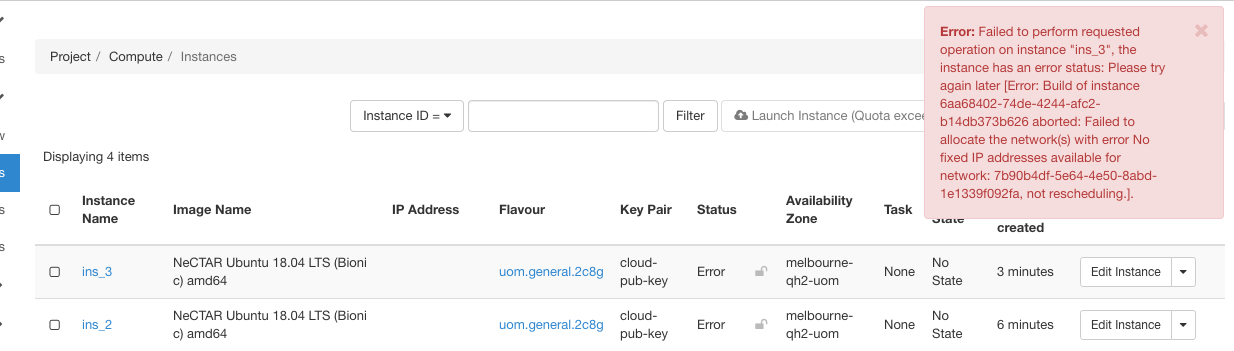
\includegraphics[width=13cm,keepaspectratio=true]{images/cloud_issue.png}
    \caption{Floating IPs issue on NeCTAR}
    \label{fig:floatingipissue}
    \end{figure}
    
    \item There is a possibility of potential data loss on the root disk \texttt{vda}. Due to this unreliability, we are not able to use 30GB storage provided by the root disk for any operation. We attached other persisted storage of 50GB and 10GB for our application and CouchDB so that we can minimize our risk of data loss. Even after that, volume snapshots are recommended. 


\end{itemize}